\documentclass{article}
\usepackage[english]{babel}
\usepackage[letterpaper,top=3cm,bottom=3cm,left=4cm,right=4cm,marginparwidth=1.75cm]{geometry}
\usepackage{amsmath}
\usepackage{graphicx}
\usepackage[colorlinks=true, allcolors=blue]{hyperref}


\title{\textbf{
\includegraphics[width=0.7\textwidth]{figures/logo}\\
    \vspace{4 cm}
    BMon: Bonsai Monitor}\\  
    \vspace{2 mm}
    Mobile and Pervasive Computing Course Project}

\author{João Antão \and João Martins}


\begin{document}
\maketitle
\vspace{2 cm}
\newpage
\tableofcontents
\newpage

\section{Introduction}
Bonsai is  the art of growing miniatures of other species by limiting the space
that the root has to grow and controlling meticulously the plant’s water intake.
Bonsai trees are more delicate than the average indoor plant, and different
species need different environments in order to achieve the wanted
appearance\,\cite{bonsai_care}. 

With this in mind, our goal with this project is to provide bonsai growers with
precise and accurate information regarding key factors of the bonsai's
environment, namely temperature, humidity, luminosity, and soil moisture. To
achieve this goal in the context of the \textbf{Mobile and Pervasive Computing}
course, we have designed and developed a microcontroller system, and a mobile
application.

The remainder of this document is organized as follows. In
Section\,\ref{sec:overview} we present a general overview of the system.
Section\,\ref{sec:architecture}, describes the system's  architecture and design
choices. In Section\,\ref{sec:mobile}, we go over the mobile application's
design and briefly explore each of its features. Furthermore, in
Section\,\ref{sec:sensors_actuators} we explore how the sensors and actuators in
our system were used to provide those features. Finally, in
Section\,\ref{sec:experiments} and Section\,\ref{sec:conclusion}, we present
respectively the experiments conducted, and our conclusions.


\section{General Overview}\label{sec:overview}
% General feature overview
From the end-user's perspective, to use our system, he would have to install one
microcontroller unit for one bonsai tree. Moreover, he would have to provide
Wi-Fi credentials in order for the unit to connect to the internet, and register
the wanted name of the bonsai tree. After the microcontroller unit is installed,
the user is able to access that unit's information in the mobile application
through the name registered previously. There, sensor data is provided and
updated periodically. Also in the application, the user will find various
editable configuration parameters.

% It requires a server?
The application and microcontroller unit exchange data through a real-time
database. As such, we need a server to hold sensor and application data, and to
handle accesses to that data. With the communication between microcontroller
unit and application being carried out through this server, it is simple
extending it to support having one user accessing many bonsai trees and one
bonsai tree being accessed by many users.

% How many microcontrollers units you need?
We have developed our prototype with one microcontroller unit for one bonsai
tree as described in Section\,\ref{sec:architecture}. However, with the
microcontroller used, it is possible to (assuming they are close to each other)
monitor up to two bonsai trees per microcontroller unit. This means that, if we
were to make this a product, we could have different models of microcontroller
units and sell them with different price tags.

% Which sensors you use and how many of them?
For our prototype, we used three different sensors: A Grove soil moisture
sensor\,\cite{sensor_moisture}; A Grove temperature and humidity sensor
(DHT11)\,\cite{sensor_dht11}; And a photoresistor to monitor the luminosity that
the tree has access to. As previously mentioned, we only developed the prototype
to monitor one bonsai tree, but if we were to extend it we could have one
microcontroller with \texttt{n} moisture sensors and one DHT11, and one
photoresistor. With \texttt{n} being the number of trees, and assuming they are
close to each other.

% Which are the interactions between the system’s elements?
The system's interactions are as follows. Sensors retrieve data from the
environment that is then registered locally in the microcontroller. Such data is
processed locally, its changes are reflected on the system's actuators.
Additionally, that data is sent to a database that the application also ha
access to. Changes on database data are reflected on the application, and thus
provided to the user.

The application also does communicate with the microcontroller (i.e., through
the cloud service provider), in our case, to send user configurations to the
microcontroller unit. The currently available configurable parameters are: 

\begin{itemize}
    \item \texttt{humidifier\_on} - boolean value that indicates whether the
    humidifier actuator should be turned when the humidity value is lower than
    \texttt{hum\_low};
    \item \texttt{cycle\_delay} - time in milliseconds to wait between each
    measurement cycle;
    \item \texttt{sync\_interval} - interval in measurement cycles between each
    database synchronization step;
    \item \texttt{hum\_high} - upper boundary for the humidity (in percentage)
    value;
    \item \texttt{hum\_low} - lower boundary for the humidity (in percentage)
    value;
    \item \texttt{lum\_high} - upper boundary for the luminosity (in percentage)
    value;
    \item \texttt{lum\_low} - lower boundary for the luminosity (in percentage)
    value;
    \item \texttt{moist\_high} - upper boundary for the soil moisture (in
    percentage) value;
    \item \texttt{moist\_low} - lower boundary for the soil moisture (in
    percentage) value;
    \item \texttt{temp\_high} - upper boundary for the temperature (in Celsius)
    value;
    \item \texttt{temp\_low} - lower boundary for the temperature (in Celsius)
    value;
\end{itemize}



\section{System Architecture}\label{sec:architecture}
% The overall architecture, including all its the components, e.g. mobile
% application, service running in the Cloud (if you need one — note that, for
% proof of concept, this service may run in your laptop), microcontroller(s),
% sensors and actuators; How the system’s components communicate and interact
% with each other (protocols); How you will implement your mobile application,
% including the server counterpart (if such element exists).


Our system consists of three main components: The microcontroller unit, the
cloud backend service (i.e., Firebase\,\cite{firebase} in our case), and the
mobile android application.These components communicate through the internet
using Wi-Fi connections (i.e., the microcontroller  unit and android phone
connect to an access point). We should also point out that the microcontroller
unit and android mobile application do not communicate directly. Instead, they
read from and write to a real-time database that is provided by the cloud
service, as can be seen in Figure\,\ref{fig:communication}.

%  We will cover in more detail each of these components in the remainder of
% this Section. 

\begin{figure}[!ht]
    \centering
    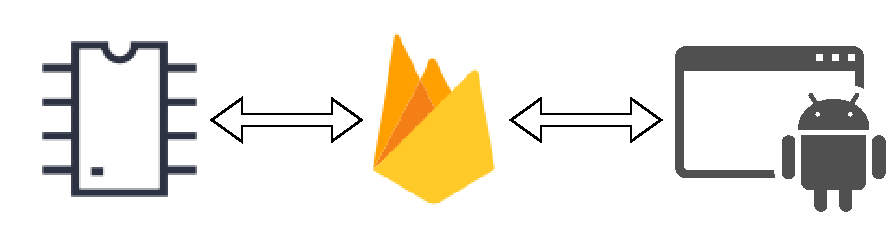
\includegraphics[width=1\textwidth]{figures/communication}
    \caption{Component communication (microcontroller unit on the left, Firebase
    in the center, and the mobile application on the right).}
    \label{fig:communication}
\end{figure}



\subsection{Cloud Backend Service}
The cloud backend service, in our case, is a central piece of our system as all
microcontroller units and applications communicate through it. With this in
mind, we start by presenting how we use it and why, in order to better
understand the design and development choices of the other components.

We have decided to use the Firebase backend service for its availability (i.e.,
being a cloud service provided by Google) and plethora of features. Furthermore,
we found its integration with the \textbf{ESP32} microcontroller simple and
straightforward\,\cite{firebase_esp32,mozbit}. More specifically, we take
advantage of its real-time database service to store the configurations provided
by the user that affect the microcontroller unit's behavior (see
Section\,\ref{sec:sensors_actuators}), and the data read from the sensors to be
accessed by the mobile application. The database scheme we used consisted of a
JSON file organized in a tree manner. Such scheme is represented in
Figure\,\ref{fig:database}.

\begin{figure}[!ht]
    \centering
    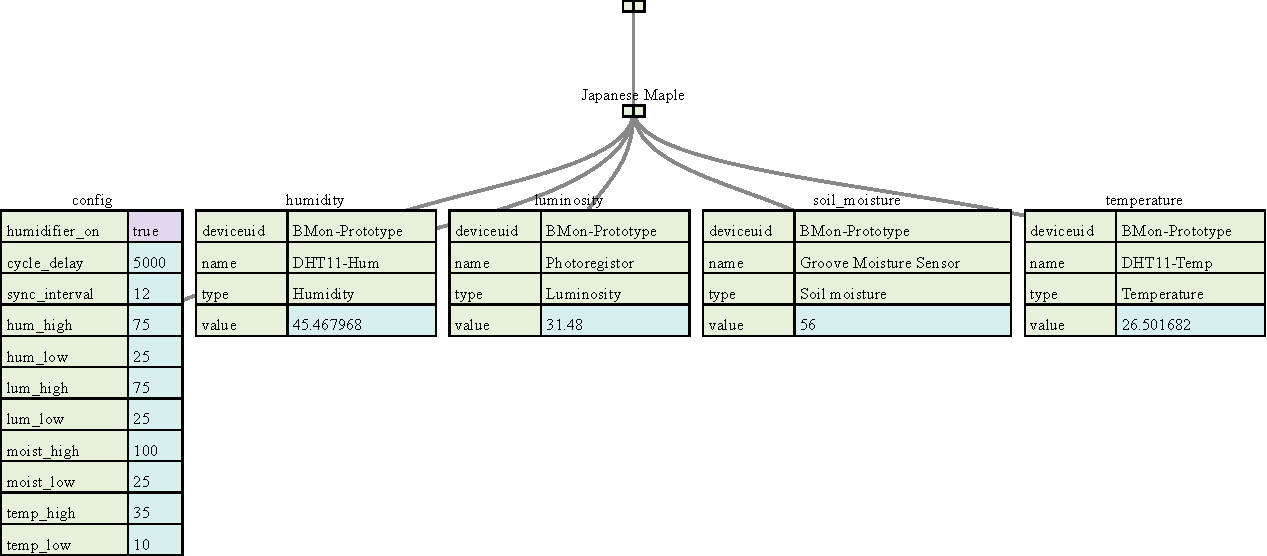
\includegraphics[width=1\textwidth]{figures/database_diagram}
    \caption{Database scheme.}
    \label{fig:database}
\end{figure}


\subsection{Microcontroller Unit}
The microcontroller unit is represented in Figure\,\ref{fig:architecture}, but
the components in the image do not match to the components used in our
prototype. The Figure is just representative of the circuit built.



\subsubsection{Microcontroller}
The microcontroller used was the \textbf{ESP32}, more specifically the
\textbf{Espressif ESP32-S2-WROVER} development board, which includes a Wi-Fi
module that allowed us to connect the unit directly to the cloud backend
service. To achieve that, we followed Fabrice Beya's
guide\,\cite{firebase_esp32} on using the Firebase library provided by
mozbit\,\cite{mozbit}. In Figure\,\ref{fig:architecture}, the development board
is represented by the big red component (sorry for the terminology).

This component is responsible for gathering the readings from all the sensors,
process those readings locally and reflect their changes on the respective LEDs
as described in Section\,\ref{sec:sensors_actuators}. Furthermore, it is
responsible for sending a weighted average of the values provided by the sensors
to Firebase's real-time database periodically. This periodicity and other
configurations can be defined by the user through the configuration available
for each plant in the database that is also periodically read by the unit.


\subsubsection{Sensors}
For our prototype, we used three different sensors: A Grove soil moisture
sensor\,\cite{sensor_moisture}; A Grove temperature and humidity sensor
(DHT11)\,\cite{sensor_dht11}; And a photoresistor to monitor the luminosity that
the tree has access to.

All the sensors are read  and their readings synced to the database
periodically. However, all readings are processed locally and can have visible
effects on the unit even before data is uploaded to the database.

\begin{figure}[!ht]
    \centering
    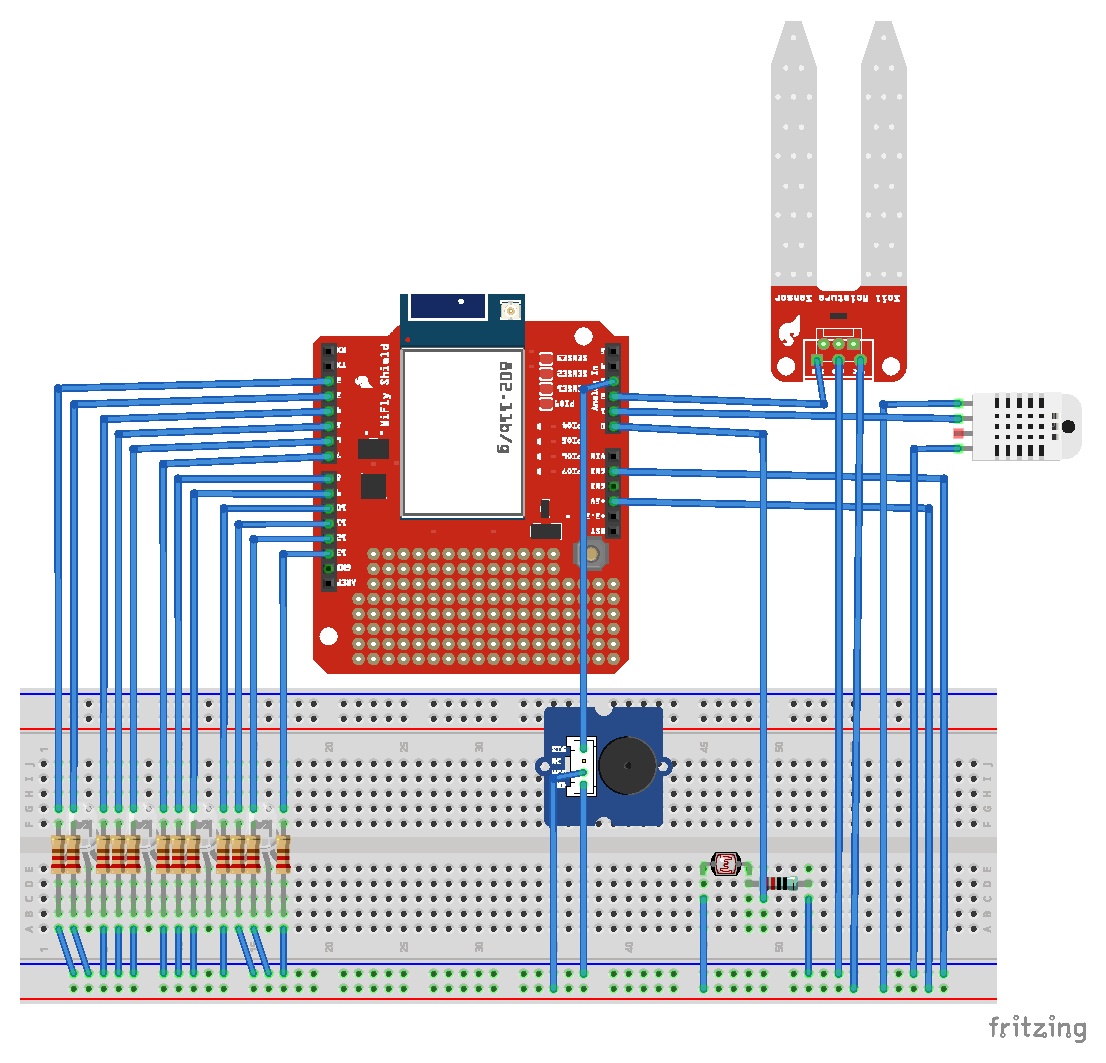
\includegraphics[width=0.7\textwidth]{figures/bmon_arch}
    \caption{Microcontroller unit circuit architecture.}
    \label{fig:architecture}
\end{figure}

\subsubsection{Actuators}
We have included two types of actuators in our prototype. More specifically, we
have RGB LEDs to display each parameter's state according to user configured
values, and a humidifier to keep the humidity around another user provided
value. These values are provided by the user through the configuration node, as
can be seen in Figure\,\ref{fig:database}.



\subsection{Mobile Application}
The system architecture also includes a mobile application which will be used to
register new bonsai to the system and at the same time act as a dashboard to the
same bonsai. The mobile application is covered in the next section.

\section{Mobile Application}\label{sec:mobile}
% Explain how you have implemented your mobile application, including the server
% counterpart (if such element exists). You must present screenshots of your
% application and all relevant implementation details.


\section{Sensing and Reacting}\label{sec:sensors_actuators}
% Explain how the system sensors and actuators are integrated within your
% application. Present a simple and short explanation of their behavior and the
% electronic schema of the connections. You must also explain the more relevant
% details of the code where the sensors and actuator signals are handled and how
% they interact. If you did not use the “real” sensors and actuators, indicate
% how you have simulated their behavior in your system.

As we have previously mentioned, our goal with this project is to provide bonsai
growers with precise and accurate information regarding key factors of the
bonsai's environment, namely temperature, humidity, luminosity, and soil
moisture. For this we have used three different sensors, namely one for soil
moisture, one for luminosity, and one for both temperature and humidity. The
general behavior of these sensors was already described in this document and, as
such, in this Section we focus on how their readings affect the system.

Values are read from the sensors periodically. After being collected, they are
added to the weighed average of all the respective environment parameter
readings. Furthermore, whenever new measurements are taken (i.e., at each cycle)
those values pass through a verification that sees whether they are dangerous or
not.

Regarding the temperature, it is measured in Celsius and the user can configure
boundaries as described in Section\,\ref{sec:overview}. If the weighted average
of the values red gets lower than \texttt{temp\_low}, then a blue LED is light
up as an alert, if the values get higher than \texttt{temp\_high} than the LED
turns red. When the temperature is in between those values, the LED remains
green.

All the other parameters are read as percentage values and the behavior of the
respective LED is the same as we just described. However, the humidity parameter
has another actuator that triggers with its value. This actuator is a humidifier
that should increase the level of humidity when turned on. Note that this is an
option and that by default, the humidifier is turned off, hence it has to be
explicitly turned on by the user. When turned on, the humidifier will only be
triggered while the humidity value is lower than \texttt{temp\_low}. We have not
integrated the humidifier on our prototype yet, but we have simulated it through
a red LED that lights up when the humidifier was supposed to be triggered. This
is represented in Figure\,\ref{fig:architecture} as a blue buzzer in the middle
of the bread board, just for purposes of demonstration.

\section{Experiments}\label{sec:experiments}
% Report the experiments you have conducted to assess the correctness and
% usability of your solution. For each experiment, always indicate its purpose,
% the assumptions made, and the tests.
Experiments conducted were only regarding the interaction between the
microcontroller unit and Firebase in order to assess whether all data was being
read and written properly by the unit.


\section{Conclusions and Lessons Learned}\label{sec:conclusion}
% Describe some of the aspects that, in your opinion, should be addressed in a
% real-world implementation of your project. Present the more relevant lessons
% that you learned from this work and some final remarks
While designing and developing the BMon system, we were faced with many design
decisions that in the end affected our overall architecture. Furthermore, we
have simplified our use cases in order to develop a functional prototype and by
doing this, we excluded interesting options and problems such as introducing
various users and bonsai trees and exploring how the interactions between these
should be laid out. If we were to work on this project on the future, exploring
a more ``decentralized'' approach that does not rely so much on the external
cloud service provider would be our goal.

This said, we have learned that there are many options to choose from when
designing a microcontroller/mobile application system that lead to different
architectures and consequently, different interaction patterns that, depending
on the use cases, sometimes are better than others.

\newpage
\bibliographystyle{IEEEtran}
\bibliography{bibliography}

\end{document}